\documentclass[12pt, a4paper]{article}
\usepackage[utf8]{inputenc}
\usepackage[T1]{fontenc}
\usepackage{geometry}
\geometry{left=2.5cm, right=2.5cm, top=2.5cm, bottom=2.5cm}
\usepackage{tikz}
\usetikzlibrary{decorations.pathreplacing}
\usepackage{graphicx}
\usepackage{amsmath, amssymb}
\usepackage{setspace}
\usepackage{hyperref}
\usepackage[
    bibstyle=numeric,
    citestyle=authoryear,
    backend=biber,
    natbib=true,
    sorting=nyt]{biblatex}
\usepackage{booktabs}
\usepackage{pgfgantt}
\usepackage{titlesec}
\usepackage{indentfirst}
\addbibresource{reference.bib}
\title{Second Year Research Proposal}
\author{Ke Jiang}
\date{}

\begin{document}

\maketitle

\vspace{1.5cm}

\noindent\textbf{Project Title:} Local Control and
Metropolitan Inefficiency: The Interaction between
Zoning and Transportation Investment\par
\bigskip
\noindent\textbf{Student's Name:} Ke Jiang\par
\medskip
\noindent\textbf{Signature:} \rule{5cm}{0.4pt} \hfill \textbf{Date:} \rule{3.5cm}{0.4pt}\par
\bigskip\bigskip
\noindent\textbf{Primary Faculty Consultant:} \rule{10cm}{0.4pt}\par
\medskip
\noindent\textbf{Signature:} \rule{5cm}{0.4pt} \hfill \textbf{Date:} \rule{3.5cm}{0.4pt}\par
\bigskip\bigskip
\noindent\textbf{Secondary Faculty Consultant:} \rule{9.5cm}{0.4pt}\par
\medskip
\noindent\textbf{Signature:} \rule{5cm}{0.4pt} \hfill \textbf{Date:} \rule{3.5cm}{0.4pt}\par

\newpage

\section{Introduction}
\subsection{Motivation}
Transportation infrastructure is a critical component of urban economic activity. It improves access to jobs and amenities and can shape the spatial structure of cities \citep{Redding2025-fr}. However, the returns to transportation infrastructure depend critically on local conditions, such as housing supply restrictions that limit density and ridership responses to new infrastructure \citep{Tsivanidis2023-hs,Severen2021-oi}. Existing literature often treats housing supply constraints as given, but in practice these constraints are frequently the result of local zoning policies. Such policies are locally determined and politically supported by incumbent residents, who value neighborhood amenities and property values \citep{Rollet2025-mk}. Although restrictive zoning may generate local benefits, it can also impose spillover costs on the broader metropolitan area and distort transportation infrasructure. This proposal therefore asks: how does local zoning distort metropolitan transportation investment decisions, what is the optimal transportation network when zoning and transportation policies are coordinated, and what are the welfare implications?

This proposal focuses in particular on transit investment decisions for two reasons. First, unlike road networks, whose benefits accrue to car commuters distributed broadly across the metropolitan network, transit investment generates returns concentrated at fixed station nodes. These returns depend critically on whether residents and employers can locate close enough to stations \citep{Hu2025-hj}. Roads, by contrast, serve car commuters across a diffuse network of routes and do not require density to be concentrated at any particular location. This node-based return structure makes transit investment especially sensitive to local zoning. Second, empirical evidence suggests that the United States has lagged behind other countries in transit infrastructure development. \cite{Freemark2023-jh} reports that U.S. transit expansion appears to have stagnated since the 1980s (fig. \ref{metro lines global}). I hypothesize that the asymmetric response of transit and road investment to local zoning may be an important factor contributing to this stagnation.

Underinvestment in transit may also generate a self-reinforcing dynamic through residential sorting. When transit is undersupplied, households substitute toward car-based commuting, which expands the feasible commuting radius and allows households to sort into more distant, lower-density locations \citep{Baum-Snow2007-zj}. As population disperses into previously undeveloped areas, newly incorporated municipalities may emerge whose residents have selected into low-density living and therefore have strong political incentives to adopt restrictive zoning that preserves the neighborhood character they moved there to enjoy \citep{Mast2024-zi}. This creates new constituencies for restrictive zoning in areas that might otherwise have remained undeveloped, further lowering metropolitan density and the ridership base for future transit expansion. In this sense, the mechanism studied in this proposal may produce not only a static inefficiency but also a path-dependent process through which metropolitan areas continue to sprawl. This process has important policy implications. Low-density sprawl requires more road infrastructure per capita, and construction and maintenance costs may become unsustainable \citep{Brueckner2000-vd}. Car dependence and long commuting distances can also increase congestion costs that are not internalized by households. Moreover, low transit investment can limit low-income households' access to job opportunities, exacerbating economic inequality \citep{Glaeser2008-xq}.


To answer the questions raised above, I plan to develop a quantitative spatial model with endogenous zoning regulation and transportation investment, following \cite{Fajgelbaum2020-yv}. The model will be calibrated to U.S. metropolitan data and used to evaluate both the existing transportation network, especially the transit network, and the counterfactual optimal network under coordinated zoning and transportation policies. I will also evaluate welfare differences between the two scenarios to estimate the potential welfare gains and identify the winners and losers from policy coordination.



\subsection{Literature Review}

This proposal draws on three interconnected bodies of literature: studies of transportation infrastructure and its evaluation, literature on zoning and land-use regulation, and research on urban sprawl and city growth patterns.

\subsubsection{Transportation Infrastructure, Optimal Structure, and Evaluation}

A large body of literature examines how transportation infrastructure shapes spatial economic patterns and how to evaluate infrastructure investments. \citet{Donaldson2025-wa} provides a comprehensive framework for evaluating transportation infrastructure impacts, emphasizing the importance of general equilibrium effects and showing how infrastructure changes affect economic activity through multiple channels. The quantitative spatial economics framework is essential for this evaluation: \citet{Redding2025-fr} surveys quantitative urban economics methods, while \citet{Redding2017-nf} details the development of quantitative spatial models that can integrate multiple dimensions of infrastructure impacts. Contemporary applications of these methods highlight that traditional benefit-cost analyses may not capture full infrastructure impacts. \citet{Severen2026-qx} describes how quantitative spatial models can evaluate transportation improvements within cities, providing practical guidance for implementation. Importantly, \citet{Fajgelbaum2021-fx} develops a framework integrating spatial epidemiology and commuting networks, demonstrating the importance of accounting for spatial structure in policy design. The returns to transit infrastructure specifically have received attention. \citet{Tsivanidis2023-hs} evaluates Bogotá's TransMilenio system and finds that transit returns depend critically on complementary policies affecting land use. \citet{Baum-Snow2000-xl} studies rail transit expansion in five U.S. cities and finds modest impacts on usage and housing values, suggesting limitations to transit investment absent other changes. \citet{Kahn2007-xc} documents significant heterogeneity in transit effects across 14 cities, with gentrification outcomes varying substantially based on local conditions like station type (walk-and-ride versus park-and-ride).

The interaction between transportation infrastructure and congestion is increasingly recognized. \citet{Akbar2023-ce} analyzes the relationship between mobility and congestion in urban India, showing how congestion affects the effectiveness of transportation improvements. \citet{Allen2022-ms} develops a general equilibrium framework with endogenous congestion to evaluate welfare impacts of transportation improvements, finding substantial variation in returns across different infrastructure investments. \citet{Kashner2025-iv} relates congestion to upzoning, showing that the effect of upzoning on housing supply depends on where upzoning occurs. Specifically, upzoning near transit stations has lower congestion effects than upzoning in other areas. My proposal contributes by modeling the endogeneity of zoning regulations and transportation investment, which are often taken as given in the literature.
\subsubsection{Zoning and Land-Use Regulation}

Zoning and land-use regulations have emerged as critical determinants of urban form and economic efficiency. The foundational work of \citet{Glaeser2002-vq} demonstrates that zoning restrictions significantly reduce housing supply elasticity, with particularly severe constraints in high-demand cities. This finding has profound implications: \citet{Hsieh2019-rx} quantifies the aggregate costs of housing constraints, estimating that zoning restrictions lowered U.S. aggregate growth by 36 percent between 1964 and 2009 by preventing the spatial reallocation of labor to high-productivity locations.

Recent work has continued this examination with new evidence and methods. \citet{Rollet2025-mk} measures winners and losers from increasing housing supply, highlighting the distributional tensions inherent in zoning reform---local residents benefit from restrictive zoning even when it imposes broader costs. \citet{Song2025-ft} estimates the effects of residential zoning on U.S. housing markets, providing detailed evidence of how zoning shapes housing supply responses. \citet{Mast2024-zi} uses electoral reforms as a source of exogenous variation in local control and finds that decentralization of land-use authority reduces housing permits by 20 percent, with larger effects in affluent areas. These results highlight how local political economy affects housing supply. Importantly, \citet{Baum-Snow2025-ml} surveys housing supply and affordability, providing context for understanding how zoning interacts with other factors affecting housing markets. A critical insight from recent work is that land-use regulations interact with transportation investment. \citet{Hu2025-hj} studies how subway expansion affects outcomes under different zoning regimes, finding that rigid land-use regulation limits the benefits of transit infrastructure. My proposal seeks to endogenize zoning regulation and investigate its spillover effects on aggregate transportation investment decisions.

\subsubsection{Urban Sprawl and City Growth}

Urban sprawl represents a fundamental concern in metropolitan economics. \citet{Brueckner2000-vd} provides the canonical analysis of sprawl causes and remedies, identifying three market failures: incomplete internalization of open-space benefits, failure to charge commuters for congestion externalities, and insufficient cost-recovery for infrastructure. \citet{Baum-Snow2007-zj}, discussed above, documents empirically how highways have driven suburban decentralization, with implications for sprawl patterns. \citet{Glaeser2003-sr} documents that sprawl is ubiquitous and continuing to expand, but is not caused by bad urban planning; rather, it reflects increasing demand for car-based living, though low-income people who cannot afford cars are left behind. My proposal seeks to explain another mechanism through which car ownership may be not only a preference but also an equilibrium outcome.

The literature collectively demonstrates that sprawl outcomes reflect a complex interaction between fundamental forces, such as population growth, rising incomes, falling transport costs, and structural changes. \citet{Cuberes2021-vo} documents urban growth shadows and access effects, showing how proximity to large metropolitan areas affects growth patterns through both competition and market-access mechanisms. \citet{Desmet2017-kc} traces the long-term evolution of U.S. settlement patterns from 1800-2000, documenting the transition toward increasingly dispersed city systems. Structural change and land use are intimately connected. \citet{Coeurdacier2022-ip} studies how structural change in the economy drives land-use changes and urban expansion. International evidence adds important insights: \citet{Zheng2013-of} documents how China's bullet trains facilitate market integration and mitigate megacity growth costs by allowing workers to access large labor markets from secondary cities. Building on these integrated insights, my proposal explores a potential mechanism that may further contribute to urban sprawl.

\section{Methodology}
\subsection{Planned Empirical Work}

The empirical part of the project will examine whether metropolitan transportation investment is shaped by the expected economic returns to transit. I plan to focus on three related hypotheses:
\begin{enumerate}
    \item Transportation investment decisions respond to the expected costs and benefits of new infrastructure.
    \item Older cities that developed extensive transit systems before widespread automobile dominance have higher returns to transit investment and therefore maintain larger transit networks, whereas newer, more car-oriented cities face lower returns.
    \item Restrictive zoning lowers the return to transit investment by limiting the density and ridership response around high-access locations.
\end{enumerate}

The main data sources will include the National Transit Database (NTD) and the Transit Explorer database, which provide information on transit volumes, revenues, investment, and opening dates. I will measure zoning constraints using housing supply elasticity estimates from \textcite{Baum-Snow2024-ii}.

\subsection{Quantitative Spatial Model}
Following \citet{Severen2026-qx}, I aim to develop a quantitative spatial model to answer the questions raised in the introduction. The model will capture the key features of metropolitan spatial structure, including heterogeneous locations, commuting patterns, and land-use decisions. It will also incorporate the institutional structure of local zoning and metropolitan transportation investment.

For now, I am considering a model in which local municipalities choose zoning policies to maximize incumbent welfare, while a metropolitan transportation authority chooses transportation investment to maximize regional net benefits, taking zoning as given. The key distortion arises from the fact that municipalities do not internalize the metropolitan-wide effects of their zoning decisions on housing supply, commuting patterns, and the return to transit investment. 
% Before delving into the full model, I first present a simplified toy model to illustrate the key mechanisms at play. (In progress and may be revised in the future)
% \subsection{Toy model}
% For simplicity, consider a monocentric model where every household commutes to the city center (CBD) to work, earning a uniform wage $w$, net of commuting cost $\tau x$, where $\tau=\tau(N,I)$ is the unit travel cost subject to travel volume and transportation investment. First, let's assume the economy is closed, such that total population $\bar{N}$ is fixed. Households arbitrage between commuting costs and housing units. There is a local municipality responsible for area $x \in (0,x_{m}]$, while for area $(x_{m},x_{f})$ there are unregulated areas, and $x_{f}$ determines the city fringe.
% \begin{figure}[htbp]
% \centering
% \begin{tikzpicture}[scale=1.1, >=stealth]

% % main city line
% \draw[thick, ->] (0,0) -- (10,0) node[right] {distance from CBD};

% % CBD
% \draw[fill=black] (0,0) circle (2pt);
% \node[below] at (0,0) {CBD};
% \node[above] at (0,0.15) {$x=0$};

% % generic location
% \draw[fill=black] (5,0) circle (2pt);
% \node[below] at (5,0) {location $x_{m}$};

% % urban boundary
% \draw[fill=black] (8,0) circle (2pt);
% \node[below] at (8,0) {urban fringe};
% \node[above] at (8,0.15) {$x_{f}$};

% % agricultural land
% % \draw[dashed] (8,0) -- (8,1.2);
% % \node[above] at (8,1.2) {$r(\bar{x})=r_A$};
% % \node[below] at (9.1,-0.35) {agricultural land};

% % commuting arrow
% \draw[<->] (0,-0.8) -- (5,-0.8);
% \node[below] at (2.5,-0.8) {local municipality};

% % city area label
% \draw[decorate, decoration={brace, amplitude=5pt}] (0,0.6) -- (8,0.6);
% \node[above] at (4,0.8) {urban land};

% \end{tikzpicture}
% \caption{A line-segment representation of the monocentric city model}
% \end{figure}
% \subsubsection{Household}
% Following \cite{Glaeser2003-sr}, I write household utility as follows:
% \begin{equation}
%   u(c,h)=c+\alpha \log h
% \end{equation}
% with budget constraint $w -\tau x=c+ hp(x)$, where $p(x)$ is the housing price. Optimal allocation of housing gives $p(x)h=\alpha$. Equilibrium implies households are indifferent across locations, such that $p'(x)h+\tau=0
% $ These two conditions pin down the housing price in terms of location $x$:
% \begin{equation}
%     P(x)=P(0)exp(-\frac{\tau}{\alpha}x)
% \end{equation}
% \subsubsection{Developer}
% Housing supply on each parcel of land is provided by competitive developers who solve:
% \begin{equation}
%     \max \pi= p S^{\gamma}-S-r
% \end{equation}
% where $S$ is structural density (housing capital per land unit), which captures housing intensity, or building height. By setting $\gamma \in (0,1)$, housing production exhibits decreasing returns to scale. In the competitive, free-entry developer market, $r(x)=p(x)S(x)^\gamma- S(x)$, which pins down the land price. Solving the developer's problem gives $s(x)=(\gamma p(x))^{1/(1-\gamma)}$. Combining housing supply and housing demand, population density is determined by:
% \begin{equation}
%     n(x)=\frac{H(x)}{h(x)}=\frac{p(x)S(x)^\gamma}{\alpha}
% \end{equation}
% \subsubsection{Local Municipality}
% The local municipality responsible for location $(0,x_{m}]$ cares about land prices and local quality of life, which is negatively correlated with density. I formulate the local municipality's problem as follows:
% \begin{equation}
%     \max_{s(x)} \int_{0}^{x_{m}} [r(x) -\omega n(x)] dx
% \end{equation}
% where $\omega$ captures the marginal disutility from density. Combined with previous conditions, this can be refined as:
% \begin{equation}
%     \max_{s(x)} \int_{0}^{x_{m}} p(x)S(x)^{\gamma}-S(x) -\omega \frac{p(x)S(x)^{\gamma}}{\alpha} dx
% \end{equation}
% The optimal structural density is $S_{m}(x)=(\gamma p(x)(1-\frac{\omega}{\alpha}))^{1/(1-\gamma)}$. To have a zoning restriction such that $S_{m}(x) < S^{\star}(x)$, we only need $\omega > 0$. Intuitively, when local residents have a preference for lower density (captured by $\omega > 0$), they choose zoning that restricts density below the unconstrained developer optimum.

% \subsubsection{Transit Infrastructure}

% Suppose a metropolitan transit authority chooses the length of a transit line by solving
% \[
% \max_{X_T}
% \int_0^{X_T} v x n_m(x)dx-F-cX_T.
% \]
% where $v$ is the value of transit accessibility (the value of unit travel cost saved per trip), and $cX_T+F$ represents the cost of building the transit line.
% Under the local municipality's zoning restriction, population density along the transit line is $n_m(x)=\frac{p(x)S_m(x)^\gamma}{\alpha}$. Solving the transit authority's problem gives the first-order condition:

% The optimal transit length is
% \[
% X_T^*
% =
% \frac{1}{\kappa}
% \log\left(\frac{vN_0}{c}\right),
% \]
% and the building condition is 
% \[
% \frac{vN_0}{\kappa}
% \left(1-\frac{c}{vN_0}\right)
% -\frac{c}{\kappa}\log\left(\frac{vN_0}{c}\right)
% \geq F
% \]
% where $\kappa=\frac{\tau}{\alpha}(1+\frac{\gamma}{1-\gamma}\frac{\omega}{\alpha})$ captures the effective density cost along the transit line, and $N_0=\frac{\left[\gamma\left(1-\frac{\omega}{\alpha}\right)\right]^{\frac{\gamma}{1-\gamma}}}{\alpha}p(0)^{\frac{1}{1-\gamma}}$ is the population density at the CBD. The optimal transit length is increasing in the value of transit accessibility, provided $vN_0>c$ and maximum net surplus is non-negative. Intuitively, $N_0$ decreases with $\omega$ (more restrictive zoning), which leads to lower population density along the transit line, lower returns to transit investment, and discourages transit expansion.
\subsubsection{Setup}
Consider a metropolitan area consisting of a finite set of locations \(S=\{1,2,\dots,N\}\). These locations are partitioned into a set of municipalities \(g\in G\), such that
\[
S=\bigcup_{g\in G} S^g, \qquad S^g \cap S^{g'}=\emptyset \quad \text{for } g\neq g'.
\]

Each location \(i\in S\) is endowed with a fixed amount of land \(\bar H_{i}\), which can be allocated between residential and commercial use:
\[
H_i^R + H_i^F \leq \bar H_{i}.
\]
Land use is further subject to zoning regulations. Let \(Z_i^R\) and \(Z_i^F\) denote the residential and commercial zoning restrictions at location \(i\). These regulations impose upper bounds on feasible development:
\[
H_i^R \leq \bar H_i^R(Z_i), \qquad H_i^F \leq \bar H_i^F(Z_i),
\]
where stricter zoning lowers the feasible density of development.

Locations are connected through a transportation network. Following \cite{Fajgelbaum2020-yv}, the generalized commuting cost between locations \(i\) and \(j\) is denoted by \(\tau_{ij}\), which depends on transportation infrastructure and congestion:
\[
\tau_{ij} = \tau_{ij}(I_{ij}, \mathbf n),
\]
where \(I_{ij}\) denotes the transportation investment between locations \(i\) and \(j\), and \(\mathbf n\) collects equilibrium traffic and transit usage, which generate congestion. The commuting cost is increasing in the quantity of commuters between \(i\) and \(j\):
\begin{align}
\frac{\partial \tau_{ij}}{\partial n_{ij}} \geq 0,
\end{align}
and $I_{ij}$ leads to a reduction in the commuting cost:
\begin{align}
\frac{\partial \tau_{ij}}{\partial I_{ij}} \leq 0.
\end{align}
Following \cite{Fajgelbaum2020-yv}, I will parametrize the commuting cost function as follows:
\begin{align}
    \tau_{jk}(\mathbf n,I)=\delta^{\tau}_{jk}\frac{(\mathbf{n})^{\rho}}{\mathbf{I}^{\gamma}}
\end{align}
There are three types of agents in the model: households, firms, and governments. Households choose where to live, where to work, and how to commute. Competitive firms choose labor and commercial land to produce a freely tradable good. Government decisions are made at two levels. Municipal governments choose local zoning regulations, while a metropolitan transportation authority chooses transportation investment for the urban area as a whole.

\subsubsection{Households}

A household chooses a residence location \(i\) and a workplace location \(j\). Conditional on these choices, the household consumes a composite tradable good \(Q_{ij}\) and residential land \(h_{ij}^R\). Preferences are given by
\[
u_{ij}(w)=\frac{B_i}{\tau_{ij}}
\left(\frac{Q_{ij}}{\beta}\right)^{\beta}
\left(\frac{h_{ij}^R}{1-\beta}\right)^{1-\beta}
v_{ij}(w),
\]
where \(B_i\) is the residential amenity at location \(i\), \(\beta \in (0,1)\), and \(v_{ij}(w)\) is an idiosyncratic preference shock.

Let \(q_i^R\) denote the rental price of residential land at location \(i\), and \(w_j\) the wage earned at workplace location \(j\). The household's budget constraint is
\[
Q_{ij}+q_i^R h_{ij}^R = w_j.
\]
Solving the within-choice consumption problem yields the indirect utility
\[
V_{ij}(w)=\frac{B_i}{\tau_{ij}}
\frac{w_j}{(q_i^R)^{1-\beta}}v_{ij}(w),
\]
up to a constant common to all choices.

\subsubsection{Firms}

At each workplace location \(j\), competitive firms produce a freely tradable good using effective labor and commercial land. Let output be given by
\[
Y_j = A_j F(L_j, H_j^F),
\]
where \(A_j\) is location-specific productivity, \(L_j\) is labor employed at location \(j\), and \(H_j^F\) is commercial land use. Firms solve
\[
\max_{L_j,H_j^F}
\; A_j F(L_j,H_j^F)-w_jL_j-q_j^F H_j^F,
\]
where \(q_j^F\) denotes the rental price of commercial land.

Profit maximization implies standard labor-demand and land-demand conditions. In equilibrium, wages and commercial rents adjust so that labor and land markets clear.

\subsubsection{Municipal Zoning Decisions}

Each municipality \(g\in G\) chooses a vector of zoning policies
\[
Z^g=\{Z_i\}_{i\in S^g}.
\]
To avoid modeling an explicit dynamic voting game, I assume municipal governments act as reduced-form representatives of incumbent residents. This captures the idea that local land-use policy is shaped by the interests of existing residents, who value neighborhood amenities, lower congestion, and higher property values, but do not internalize metropolitan-wide effects on housing supply, commuting, or transit efficiency.

Accordingly, municipality \(g\) solves
\[
\max_{Z^g} \; W^g=\sum_{i\in S^g} \omega_i u_i(Z^g, Z^{-g})
\]


\subsubsection{Optimal Transportation Investment}

A metropolitan transportation authority chooses investment for the region as a whole. Taking local zoning as given, the authority solves
\[
\max_{I_{jk}} \; W=\sum_{i} \omega_{i} \sum_{j} N_{ij} U_{ij}(Q_{ij}, h_{ij}^R)
\]
subject to:
\begin{align}
    \sum_{j,k} \delta_{jk} I_{jk} & \leq K, \\
    0 \leq \underline{I_{jk}} \leq I_{jk} & \leq \bar{I_{jk}} \leq \infty
\end{align}
Where $U_{ij}(Q_{ij}, h_{ij}^R)$ represents the utility of a household living in location $i$ and working in location $j$, and $N_{ij}$ is the number of such households. 


\subsubsection{Equilibrium}

A decentralized equilibrium consists of
\[
\left\{
q_i^R, q_i^F, w_j, H_i^R, H_i^F, L_j, Z^g, I^R, I^T
\right\}_{i,j\in S,\, g\in G}
\]
such that:

\begin{enumerate}
    \item Households choose residence and workplace location to maximize utility.
    \item Firms choose labor and commercial land to maximize profits.
    \item Each municipality chooses zoning to maximize incumbent resident welfare.
    \item The metropolitan transportation authority chooses road and transit investment to maximize regional net benefits, taking zoning as given.
    \item Residential land, commercial land, and labor markets clear.
\end{enumerate}

\subsubsection{Inefficiency and the Source of Sprawl}

The main distortion in the model arises from a mismatch in governance scales. Zoning is chosen locally by municipalities that represent incumbent interests, while transportation is chosen at the metropolitan level. Municipalities have incentives to restrict development in high-access locations in order to preserve local amenities and limit congestion. However, they do not internalize the broader metropolitan costs of such restrictions, including higher housing prices, greater job-housing separation, and lower returns to public transit investment.

As a result, restrictive zoning can prevent transportation improvements---especially transit investments---from translating into higher-density development near well-connected locations. Growth is instead pushed toward lower-cost, more distant areas, contributing to urban sprawl. In this sense, sprawl in the model is not simply a reflection of geography or household preferences, but may emerge as an inefficient equilibrium outcome of fragmented land-use regulation combined with metropolitan transportation investment.

\subsubsection{Efficient Benchmark: Planner's Problem}
Now, for a planner who chooses zoning and transportation investment jointly to maximize metropolitan welfare, the problem can be written as
\[
\max_{Z^g, I_{jk}} \; W=\sum_{i} \omega_{i} \sum_{j} N_{ij} U_{ij}(Q_{ij}, h_{ij}^R)
\]
subject to:
\begin{align}
    \sum_{j,k} \delta_{jk} I_{jk} & \leq K, \\
    0 \leq \underline{I_{jk}} \leq I_{jk} & \leq \bar{I_{jk}} \leq \infty, \\
    \sum_{j} N_{ij} h_{ij}^R & \leq   H_i^R, \\
    \sum_{i} \sum_{j} N_{ij} & = L, \\
    \sum_{i} \sum_{j} N_{ij} Q_{ij} & = \sum_{j} A_j F(L_j, H_j^F), \\
    H_i^R + H_i^F & \leq \bar H_i \
 \end{align}
\section{Expected Outcome}
I expect to use my model to quantify the existing U.S. metropolitan transportation network and construct the counterfactual optimal transportation network under coordinated zoning and transportation policies. I will also evaluate the welfare distribution and differences between the two scenarios to estimate how much welfare improvement can be achieved and identify the winners and losers.



\printbibliography
\begin{figure}[htbp]
    \centering
    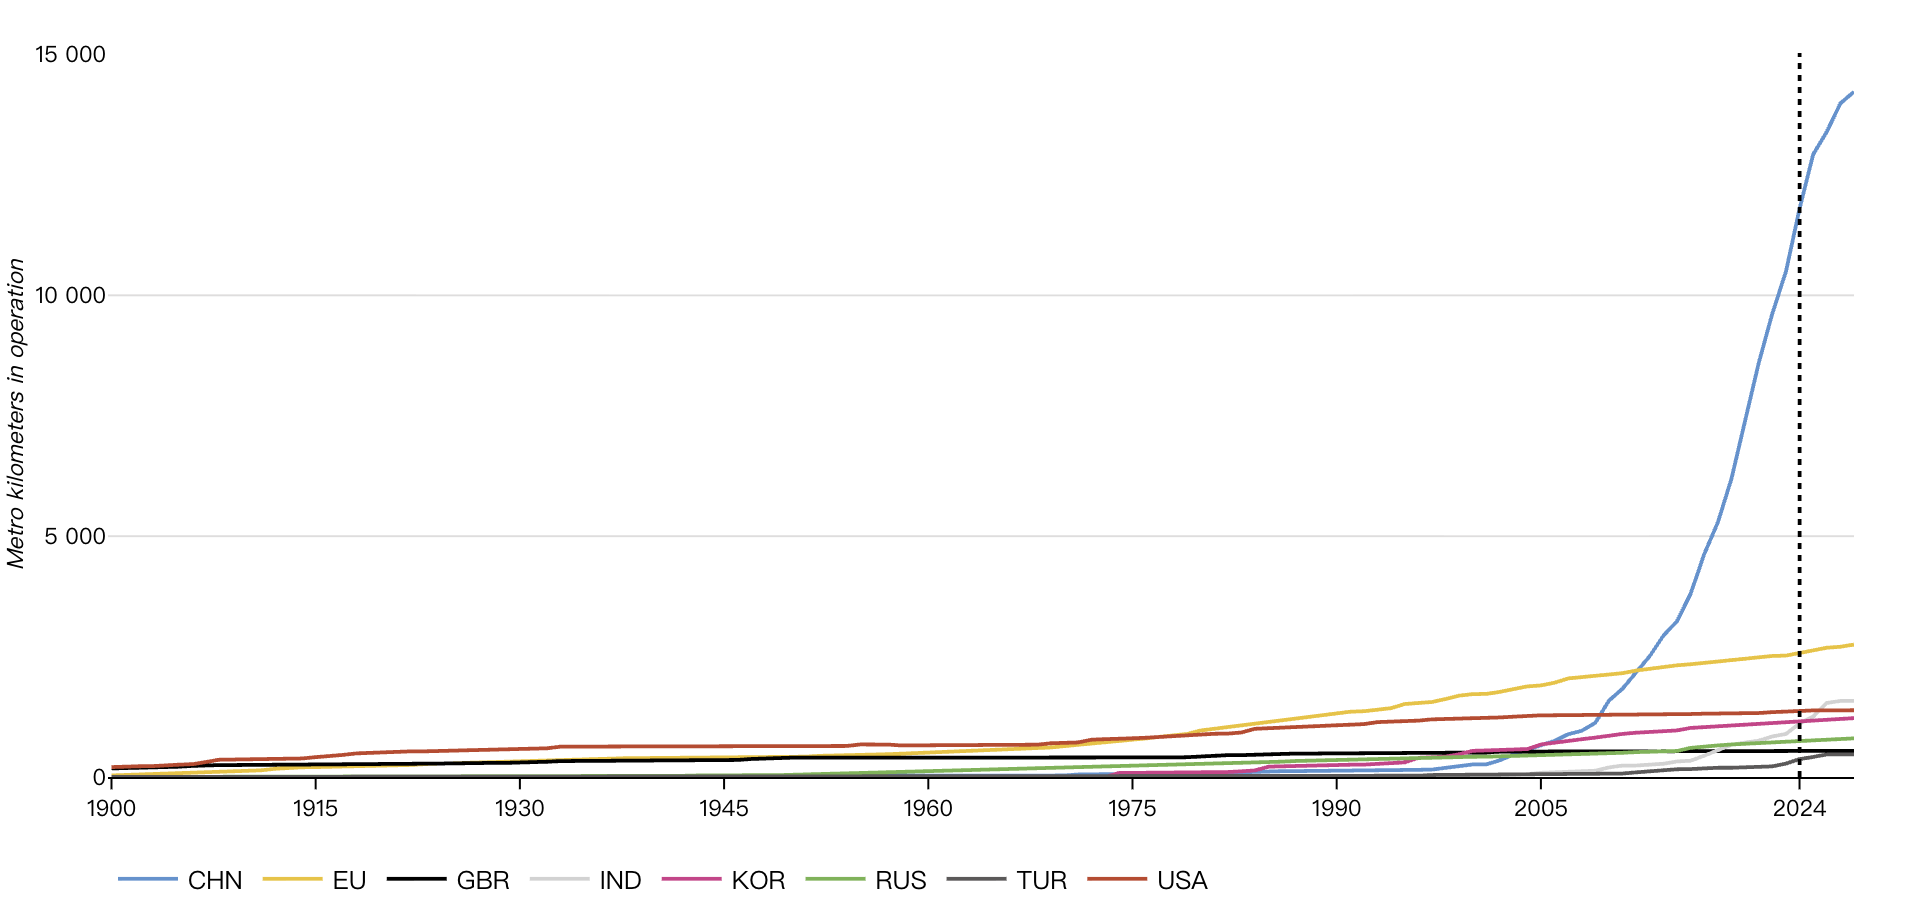
\includegraphics[width=1\linewidth]{Metro lines Global.png}
    \caption{Metro kilometers in operation}
    \label{metro lines global}
\end{figure}
\newpage
\section{Work Plan}

The project runs from May~13 to August~3, 2026, spanning twelve weeks
and approximately 57 working days (excluding Memorial Day, May~25, and
Independence Day, July~4). Work is organized in three overlapping phases.
\textbf{Phase~1} (Weeks~1--5) covers model specification and coding;
the model structure determines what data series are needed, so data
collection begins only once the model is sufficiently specified.
\textbf{Phase~2} (Weeks~3--10) covers data collection, cleaning, and
model calibration; data work and model coding run in parallel during
Weeks~3--5 and feed into calibration from Week~7 onward.
\textbf{Phase~3} (Weeks~10--12) covers counterfactual simulations and
writing. Model development and data work may iterate if calibration
reveals gaps in data coverage or model specification.

\subsection*{Activities}

\begin{table}[htbp]
\centering
\caption{Activities and Time Commitment}
\begin{tabular}{clcc}
\toprule
\textbf{\#} & \textbf{Activity} & \textbf{Weeks} & \textbf{Working Days} \\
\midrule
1 & Model specification and theoretical derivations  & W1--W3   & 13 \\
2 & Data requirements specification and collection   & W3--W5   & 18 \\
3 & Data cleaning and descriptive analysis           & W6--W8   & 12 \\
4 & Model coding and numerical solution algorithm    & W3--W5   & 13 \\
5 & Model calibration and validation                 & W7--W10  & 16 \\
6 & Counterfactual simulations and welfare analysis  & W10--W11 & 10 \\
7 & Writing and revisions                            & W10--W12 & 12 \\
\midrule
  & \textbf{Total (accounting for overlap)} & \textbf{12 weeks} & \textbf{$\approx$57 days} \\
\bottomrule
\end{tabular}
\end{table}

\noindent\textit{Note: Activities~2 and~4 run in parallel during Weeks~3--5.
Activity~5 draws on both the coded model (Activity~4) and cleaned data
(Activity~3), and therefore begins only after both are sufficiently
advanced.}

\subsection*{Milestones}

\begin{table}[htbp]
\centering
\caption{Project Milestones}
\begin{tabular}{cllp{8.5cm}}
\toprule
\textbf{M\#} & \textbf{Date} & \textbf{Day} & \textbf{Deliverable} \\
\midrule
M1 & May~30  & 13 & Model fully specified; equilibrium conditions and
                    key equations derived; data requirements identified \\
M2 & June~13 & 23 & Model coded and numerically solved;
                    all datasets collected \\
M3 & July~3  & 37 & Data cleaned; descriptive statistics and
                    stylized facts documented \\
M4 & July~18 & 47 & Model calibrated to U.S.\ metropolitan data;
                    fit validated \\
M5 & July~25 & 52 & Counterfactual simulations and welfare
                    calculations complete \\
M6 & Aug~3   & 57 & Summer paper draft submitted to faculty advisor \\
\bottomrule
\end{tabular}
\end{table}

\subsection*{Schedule}

\begin{figure}[htbp]
\centering
\begin{ganttchart}[
    hgrid,
    vgrid={*{11}{dotted}},
    x unit=0.92cm,
    y unit title=0.70cm,
    y unit chart=0.68cm,
    title label font=\small\bfseries,
    title height=1,
    bar label font=\small,
    bar height=0.55,
    bar label node/.append style={align=right, text width=4.6cm}
]{1}{12}
\gantttitle{May}{3}
\gantttitle{June}{4}
\gantttitle{July / Aug}{5} \\
\gantttitlelist{1,2,3,4,5,6,7,8,9,10,11,12}{1} \\
\ganttbar[bar/.style={fill=blue!40, rounded corners=2pt}]%
    {1.\ Model specification}{1}{3} \\
\ganttbar[bar/.style={fill=green!50, rounded corners=2pt}]%
    {2.\ Data collection}{3}{5} \\
\ganttbar[bar/.style={fill=green!50, rounded corners=2pt}]%
    {3.\ Data cleaning \& descriptives}{6}{8} \\
\ganttbar[bar/.style={fill=blue!40, rounded corners=2pt}]%
    {4.\ Model coding \& solution}{3}{5} \\
\ganttbar[bar/.style={fill=blue!40, rounded corners=2pt}]%
    {5.\ Model calibration}{7}{10} \\
\ganttbar[bar/.style={fill=orange!55, rounded corners=2pt}]%
    {6.\ Counterfactual simulations}{10}{11} \\
\ganttbar[bar/.style={fill=gray!50, rounded corners=2pt}]%
    {7.\ Writing \& revisions}{10}{12}
\end{ganttchart}
\caption{Summer work plan, May~13--August~3, 2026. Week numbers run from
Week~1 (May~13) to Week~12 (July~28--August~1); the submission deadline
of August~3 is the first working day of Week~13.
\textit{Blue}: model activities (1, 4, 5);
\textit{green}: data activities (2, 3);
\textit{orange}: simulation (6);
\textit{gray}: writing (7).
Activities~2 and~4 occupy the same weeks (W3--W5) and run in parallel.}
\label{fig:workplan}
\end{figure}

\end{document}
